% !TeX spellcheck = da_DK
\section{Systemets opbygning}
\begin{figure}[H]
	\centering
	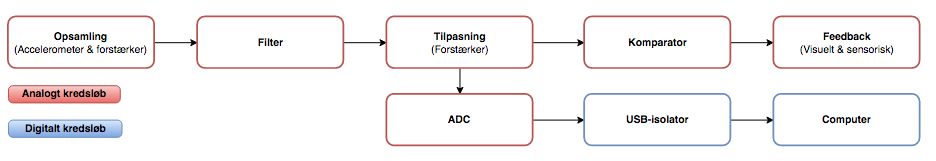
\includegraphics[scale=0.47]{figures/Blokdiagram.jpg}
	\caption{Her ses et blokdiagram af systemets opbygning}
	\label{Blokdiagram}
\end{figure}

Opsamlingsblokken indeholder accelerometret samt en forstærker, der opsamler og forstærker det biologisk signal. %Det biologiske signal, der opnås fra accelrometeret, skal forstærkes, eftersom de opfangede signalerne er små. Forstærkningen vil derfor gøre filtreringen mere præcis. Herefter benyttes et højpas filter for at frasortere den støj, der kommer fra tyngdekraften. 
I filterblokken anvendes et lavpasfilter for at frasortere støj fra frekvenser over 45 Hz. Grunden til at disse frekvenser kan frasorteres er, at det målte signal ligger under 45 Hz. Efter filtreringen af signalet benyttes en variabel forstærker for at tilpasse signalets amplitude til ADC’en og komparatoren, hvilket er vist som en tilpasnings blok på \figref{Blokdiagram}. Signalet ledes herefter videre i et analogt og digitalt kredsløb. I det analoge kredsløb kommer signalet først gennem en komparator, som skal sammenligne det optagede signal med en tærskelværdi, så den rigtige feedback kan gives til patienten ift. valgt sværhedsgrad. Feedbacken gives til patienten i form af dioder og vibratorer. I det digitale kredsløb ledes signalet ind i en ADC, som konverterer det analoge signal til et digitalt signal. Herefter ledes det digitale signal ind i en USB-isolator, der sikre patientens sikkerhed samt eliminerer lækstrøm. Til sidst overføres det digitale signal til en computer, hvor signalet herefter kan databehandles og gemmes.